%!TEX root = ../Studienarbeit.tex

\chapter{Technische Grundlagen}

\section{Bluetooth}

\subsection{Allgemein}

Bluetooth ist ein Kurzstreckenkommunikationssystem, bei welchen die Hauptmerkmale auf Robustheit, einen geringen Stromverbrauch und geringe Kosten gelegt wurde. Bluetooth wir in zwei Kategorien aufgeteilt. Die erste Kategorie ist \ac{BBR}. Die zweite Kategorie ist \ac{BLE}. Beide Kategorien beinhalten dabei Mechanismen, um Bluetooth-Geräte zu entdecken, einen Verbindungsaufbau durchzuführen sowie eine Verbindung herzustellen. Das Augenmerk bei \ac{BLE} Produkten liegt dabei auf einen niedrigen Stromverbrauch, welche durch eine geringere Datenrate und eine geringere Einschaltdauer während den Datenaustausch als bei \ac{BBR} realisiert wird. Die Übertragungsrate bei \ac{BLE} in der physikalischen Schicht beträgt 2~MB/s. Zu beachten ist, dass ein Bluetooth-Controller entweder nur \ac{BLE}, \ac{BBR} oder beide Bluetooth-Kategorien unterstützen kann. \cite[S.~187]{bluetoothCore}

Die Übertragungsfrequenz von \ac{BLE} ist im lizenzfreien 2.4~GHz ISM-Band von 2402~MHz bis 2480~MHz \cites[S.~4]{siliconBLE}[S.~190]{bluetoothCore}. Das Frequenzband ist in 40 physikalische Kanäle mit jeweils einer Bandbreite von 2~MHz aufgeteilt, wie in Abbildung \ref{fig:frequenzbandBLE} zu sehen ist \cite[S.~190]{bluetoothCore}. Drei dieser 40 physikalischen Kanäle sind für das sogenannte Advertising vorhanden \cite[S.~190]{bluetoothCore}, welches für die Geräteentdeckung, den Verbindungsaufbau und für das Broadcasting von Nachrichten vorhanden ist \cite[S.~4]{siliconBLE}. Die restlichen Kanäle sind für eine allgemeine Datenübertragung vorhanden \cite[S.~190]{bluetoothCore}. Zusätzlich zu der Aufteilung des Frequenzbandes in Kanäle werden Kanäle in Zeiteinheiten aufgeteilt, welche Events genannt werden \cite[S.~190]{bluetoothCore}. Daten werden in Paketen innerhalb eines Events übertragen. Zusätzlich wird bei der Übertragung von Daten Frequenzhopping betrieben, welches zu Beginn jedes Events stattfindet \cite[S.~190f.]{bluetoothCore}. 

\todo[inline]{Bild anpassen und schreiben, abgewandelt von ...}
\begin{figure}[h]
\centering
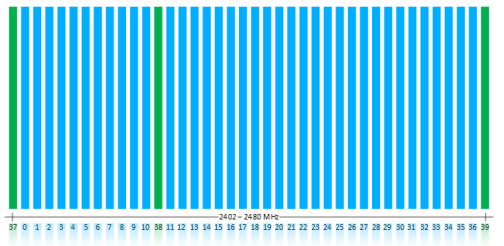
\includegraphics[height=.3\textwidth]{frequenzband}
\caption{Frequenzband mit Kanälen von \ac{BLE} \cite[S.~4]{siliconBLE}}
\label{fig:frequenzbandBLE}
\end{figure}

Die Kompatibilität zwischen Bluetooth-Geräten wird durch sogenannte Profile sichergestellt. Profile beschreiben dafür Funktionen und Eigenschaften von jeder Schicht im Bluetoothsystem \cite[S.~277]{bluetoothCore}. Ebenso werden die benötigten Nachrichten und Prozeduren für die verwendeten Profile durch die Bluetooth \ac{SIG} spezifiziert \cite[S.~1241]{bluetoothCore}.

Bluetooth-Geräten werden unterschiedliche Rollen zugewiesen. Dafür gibt es die Rollen Observer, Broadcaster, Central und Peripheral. Ein Gerät in der Rolle Broadcaster verschickt Advertising-Pakete und ein Gerät welches nur Advertising-Pakete empfangen kann hat die Observer Rolle. So kann eine einseitige Kommunikation zwischen Geräten mittels Advertising-Paketen erfolgen. Eine andere Art der Kommunikation ist mittels einer Verbindung bei dem das Initiatorgerät eine Verbindungsanfrage eines Broadcastergeräts annimmt. Daraufhin bekommt das Initiatorgerät die Rolle Central und das Gerät welches ursprünglich in der Rolle Broadcaster war, die Rolle Peripherial. Anzumerken ist, dass ein Gerät zu jeder Zeit mehrere Rollen unterstützen kann, welche jedoch alle der Bluetooth-Controller unterstützen muss. \cite[S.~190f., S.~278, S.~1246ff.]{bluetoothCore}

\subsection{Benötigte Komponenten eines \ac{BLE}-Geräts}

Ein \ac{BLE}-Gerät benötigt einen Mindestumfang an Funktionen damit es laut Bluetooth \ac{SIG} \ac{BLE} kompatibel ist. In Abbildung \todo{Referenz hinzufügen} sind die benötigten Funktionen und deren Zusammenspiel durch ein Schichtenmodell dargestellt. Die Funktionen können dabei in einen Hostteil und einen Controllerteil aufgeteilt werden. Im Hostteil befinden sich die Funktionen \ac{L2CAP}, \ac{GAP}, \ac{ATT}, \ac{GATT}, \ac{SDP} und \ac{SMP}. Im Controllerteil befinden sich die Funktionen \ac{PHY} und \ac{LL}. Die Kommunikation zwischen den Hostteil und dem Controllerteil finden mittels des \ac{HCI} statt \cite[S.~1735]{bluetoothCore}. \cite[S.~193]{bluetoothCore}

\todo[inline]{Bild erstellen}

In den nachfolgenden Unterkapiteln werden die wichtigsten Informationen jeder benötigten Funktion von \ac{BLE} beschrieben.

\subsubsection{\acf{PHY}}
Die physikalische Schicht in \ac{BLE} ist zum Verschicken und erhalten von Paketen über eines der physikalischen Funkkanäle verantwortlich. \cite[S.~209]{bluetoothCore}

\subsubsection{\acf{LL}}
Die Verbindungsschicht im \ac{BLE}-System besteht aus mehreren Komponenten. Eine Komponente ist für die Erstellung, Modifizierung und das Freigeben von logischen Verbindungen zuständig. Eine weitere Komponente ist für das Kodieren und Dekodieren von Bluetooth Paketen zuständig. Auch gibt es eine Komponente welche für die Datenflusskontrolle, die Datenbestätigung und für die Wiederübertragung von Paketen zuständig ist. Die letzten Komponenten in der Verbindungsschicht ist für den Zugriff auf das Radiomedium zuständig. Dafür gibt es einen Scheduler, welcher Zeitschlitze des physikalischen Mediums an die höherliegenden Dienste verteilt. \cite[S.~207f.]{bluetoothCore}

\subsubsection{\acf{HCI}}
Das \acl{HCI} stellt die Möglichkeit bereit, dass der Hostteil die Funktionen des Controllerteil erreichen kann. Die Übertragung des \ac{HCI} kann dabei wahlweise mittels USB, UART oder anderen Bussystemen stattfinden. \cite[S.~1735f.]{bluetoothCore}

\subsubsection{\acf{L2CAP}}
Das \acl{L2CAP} ist die Schicht im \ac{BLE}-Stack, welches eine kanalbasierte Abstraktion zu den Applikationen und Diensten der höheren Schichten bereitgestellt. Diese Schicht kümmert sich zusätzlich, um die Segmentierung, den Zusammenbau, das Multi- und Demultiplexing von Daten auf einer beziehungsweise mehreren logischen Verbindungen. \cite[S.~195, S.~1013]{bluetoothCore}

\acl{L2CAP} baut dabei auf dem Konzept von logischen Kanälen auf, wobei jeder Endpunkt eines logischen Kanals einen eindeutigen \ac{CID} hat \cite[S.~1021]{bluetoothCore}. Die logischen Kanäle werden über logische Verbindungen der \ac{LL}-Schicht übertragen \cite[S.~1013]{bluetoothCore}.

\subsubsection{\acf{GAP}}
Das \acl{GAP} beschreibt die Basisfunktionalitäten welche ein \ac{BLE}-Gerät benötigt \cite[S.~207]{bluetoothCore}. Dabei werden auch alle, in diesem Kapitel vorgestellten Schichten als Mindestanforderung aufgelistet und die alle benötigten Fähigkeiten die eine \ac{BLE}-Rolle benötigt \cite[S.~277f., S.~1241]{bluetoothCore}. 

Weitere wichtige Eigenschaften die in \ac{GAP} definiert sind, ist zum einen die Bluetooth-Geräteadresse. Diese Geräteadresse wird verwendet, um ein Bluetooth-Gerät eindeutig zu identifizieren. Eine weitere Eigenschaft, welche in \ac{GAP} definiert wird, ist der Gerätename. Dieser Name ist eine benutzerfreundliche Zeichenfolge der an entfernten Geräten angezeigt wird. Der Gerätename kann bis zu 248~Byte lang sein und sollte in UTF-8 kodiert sein. Es muss davon ausgegangen werden, dass ein Gerät nur die ersten 40 Zeichen verwenden kann. \cite[S.~1251ff.]{bluetoothCore}

Damit eine Verfolgung von Geräteadressen minimiert werden kann, gibt es in \ac{BLE} zwei Arten von Geräteadressen. Zum einen eine sich verändernde öffentliche Adresse, welche an allen \ac{BLE}-Geräte verschickt wird. Zum anderen gibt es sich nicht verändernde private Adressen, welche von Geräten ausgerechnet werden kann, welche schon einmal eine Verbindung mit dem Gerät aufgebaut haben. Damit können Geräte, welche schon einmal mit einem anderen Gerät verbunden waren, überprüfen, ob es sich um ein bereits bekanntes Gerät handelt. \cite[S.~18]{siliconBLE}

Auch wird in \ac{GAP} beschrieben, wie der Bluetooth-Pin für eine Authentifizierung zweier Geräte im Verbindungsmodus aufgebaut sein muss. Diese Pin ist sechs Zeichen lang und besteht aus Ziffern. \cite[S.~1253]{bluetoothCore}

Zu guter Letzt, beschreibt \ac{GAP} noch die verschieden Sicherheitsmodi, welche durch die verschiedenen \ac{BLE}-Rollen implementiert sein müssen \cite[S.~1337]{bluetoothCore}.

\subsubsection{\acf{SDP}}
\ac{SDP} stellt die Möglichkeit bereit, die verfügbaren Dienste und die zugehörigen Merkmale eines Bluetooth-Geräts für entfernte Geräte sichtbar zu machen \cite[S.~1173]{bluetoothCore}. Dabei pflegt das Gerät, welches \ac{SDP} bereitstellt, eine Liste aller Dienste und Merkmale des Geräts \cite[S.~1177]{bluetoothCore}.

\subsubsection{\acf{SMP}}
\ac{SMP} definiert Methoden zum Verbindungsaufbau und zum Schlüsselaustausch zwischen Bluetooth-Geräten \cite[S.~1554]{bluetoothCore}. Die gerätespezifischen Schlüssel, werden für die Identifizierung von Geräten und für den verschlüsselten Datenaustausch zwischen Geräten verwendet \cites[S.~1556]{bluetoothCore}[S.~18]{siliconBLE}.

Der Verbindungsaufbau und der dazugehörige Schlüsselaustausch für die Identifizierung der Geräte erfolgt in 3 Phasen. Die erste Phase ist die Anfrage für einen Verbindungsaufbau. Die zweite Phase, nach einer erfolgreichen Anfrage, ist die Generierung eines Schlüssels mit einer kurzen oder langen Lebenszeit. Die letzte Phase ist die Bereitstellung der generierten Schlüssel an die Gegenstelle. \cite[S.~1556]{bluetoothCore}

Zu beachten ist, dass es verschiedene Möglichkeiten gibt einen Verbindungsaufbau herzustellen, der abhängig von den Sicherheitsansprüchen der Anwendung definiert werden kann \cite[S.~18]{siliconBLE}.

\subsubsection{\acf{ATT}}
\ac{ATT} ist ein Teilnehmer-zu-Teilnehmer Protokoll zwischen zwei Geräten \cite[S.~206]{bluetoothCore}. \ac{ATT} definiert dabei zwei Rollen, den Client und den Server \cite[S.~1410]{bluetoothCore}. \ac{ATT} erlaubt es Geräten -- Clients -- kleine Werte -- sogenannte Attribute \cite[S.~279]{bluetoothCore} -- zu lesen, zu schreiben und zu entdecken, welche sich auf dem Gerät mit der Rolle Server befinden \cite[S.~1409]{bluetoothCore}. Ein Gerät kann simultan in der Rolle Server und Client sein \cite[S.~279]{bluetoothCore}.

Ein Attribut besteht jeweils aus drei Eigenschaften. Die erste Eigenschaft ist der Attribut-Typ, welcher durch eine \acf{UUID} definiert wird und in \ac{SDP} definiert sind. Die zweite Eigenschaft ist der Attribut-Handle. Der Attribut-Handle ist ein einzigartiger Identifikator für ein Attribut auf einem Gerät mit der Server-Rolle. Dadurch das Handle ist das Attribut eindeutig auf dem Gerät definiert. Die letzte Eigenschaft eines Attributs sind die Berechtigungen, welche durch eine höhere Schicht definiert werden muss. \cite[S.~1410ff.]{bluetoothCore}

Attribut-Handles haben eine Länge von 16~Bit und können durch weitere spezielle Attribute gruppiert werden \cite[S.~1412f.]{bluetoothCore}. Die Entdeckung aller vorhandenen Attribute eines Servers durch einen Client erfolgt durch eine höhere Schicht des \ac{BLE}-Stacks \cite[S.~1410]{bluetoothCore}.

Die hinterlegten Werte eines Attributs bestehen aus einem Oktett-Array mit einer fixen oder variablen Länge \cite[S.~1413]{bluetoothCore}.

\subsubsection{\acf{GATT}}

